\section{Improved EMO Algorithm for the VNFPP}
\label{sec:optimisation}
In this section we propose a new algorithm for the VNFPP that can find high quality solutions to large scale VNFPPs. There are three key components of our algorithm: 
\begin{enumerate}
    \item A novel parallel metaheuristic that efficiently searches the VNFPP solution space.
    \item A genotype-phenotype solution representation that incorporates domain knowledge to improve expected solution quality.
    \item A novel initialization operator that ensures a diverse initial pool of feasible solutions.
\end{enumerate}
\pref{fig:overview} provides an overview of how these components work together. In the first stage, \textit{preprocessing}, the algorithm decomposes the multi-objective problem into subproblems and generates data structures that aid in efficient optimization. In the second stage, \textit{optimization}, the algorithm finds solutions to each subproblem in parallel.

The remainder of this section discusses each component of the algorithm in detail. First we discuss the core optimization algorithm and the ways it improves upon from existing parallel metaheuristics in \pref{sec:core_algorithm}. Next we describe the tailored solution representation we use to aid the search process in \pref{sec:gp_mapping}. Finally, in \pref{sec:operators} we discuss the initialization and local search operators used in this work. 

\begin{figure}
    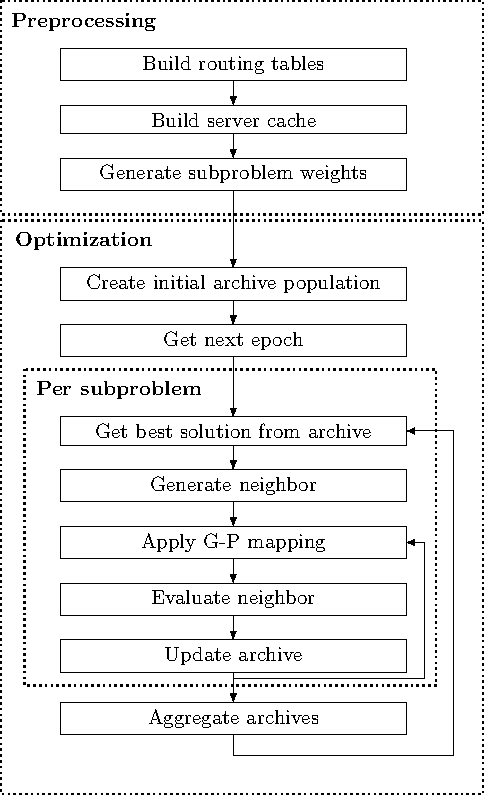
\includegraphics{figures/operators/alg_flowchart}
    \caption{A high level overview of our proposed algorithm.}
    \label{fig:overview}
\end{figure}

\subsection{Novel Parallel Metaheuristic}
\label{sec:core_algorithm}

\begin{algorithm}[t!]
	
	\KwData{Subproblems per epoch $N^s$, Number of processes $L$, Weight vectors $W = \{W^1, ..., W^N\}$, Max evaluations $T$, Number of objectives $M$}

    $N^E \gets \lceil \abs{W} / N^s \rceil$ \tcp{Number of epochs}
    $T^W \gets (T - \abs{A}) / \abs{W}$ \tcp{Evaluations per weight} 

    \tcc{Evaluate initial solutions}
    $A' \gets \textsc{Initialize}$
	\For{$s \in A'$} {
        $s_{obj} \gets \textsc{Evaluate} (s)$
	}
    $A \gets$ Non-dominated pop. of $A'$

    \For{$e \gets 0$ \KwTo $N^E$} {

        $i_f \gets e \cdot N^s$ \tcp{Index of first weight}
        $i_l \gets \min(i_f + N^s, \abs{W})$ \tcp{Index of last weight}

        \Parallel{$\ell$ in $\{W_{i_f}, ... W_{i_l}\}$} {
            $A_\ell \gets \emptyset$ \tcp{Process archive}

            \tcp{Best solution found for weight}
            $s \gets \underset{x \in A}{\argmax}\ g \left( x\ |\ W_\ell \right)$

            $A_\ell \gets A_\ell \cup s$

            $t \gets 0$ \tcp{Evaluation counter}

            \While{$t < T^W$} {
                \tcc{Get neighbouring solution}
                $s^n \gets \textsc{GenNeighbour}(s)$

                $s^n_{obj} \gets \textsc{Evaluate} (s^n)$

                $t \gets t + 1$

                \tcc{Update process archive}
                $A_\ell \gets$ Non-dominated pop. of $A_\ell \cup s^n$

                \tcc{Accept improving solutions}
                \If{$g\left(s^n | W_\ell \right) < g \left(s | W_\ell \right) $}{
                    $s \gets s^n$
                }
            }
        }

        $A \gets$ Non-dominated pop. of $(\bigcup_\ell^L A_\ell)$
    }

	\caption{Our proposed decomposition based parallel multi-objective local search algorithm.}
	\label{alg:simple_pplsd}
\end{algorithm}

It is well known that the Pareto front of a problem can be approximated by solving a diverse set of scalar optimization subproblems. For example, given the multi-objective optimization problem:
\begin{equation}
    minimize\ F(x) = (f_1(x), ..., f_m(x))^\intercal
    \label{eq:mop}
\end{equation}
where $x \in \Omega$ and $\Omega$ is the decision space, $F: \Omega \implies R^m$ consists of $m$ real valued objective functions. Provided the objectives in \pref{eq:mop} contradict each other, no point in $\Omega$ minimizes all objectives simultaneously. However, given a weight vector $\mathbf{\lambda} = \{\lambda^1, ... \lambda^n\}$ (where $\lambda_i \geq 0 \forall i = 1,\cdots,m$ and $\sum_{i=1}^m \lambda_i = 1$) and a utopian point ((i.e. $z_i^* = min \left\{f_i(x) | x \in \Omega \right\}$)),(i.e. $z_i^* = min \left\{f_i(x) | x \in \Omega \right\}$) the optimal solution to the Tchebycheff \textit{scalar} optimization problem:
\begin{equation}
    minimize\ g^{tc}(x | \lambda, z^*) = \max_{1 \leq i \leq m} \left\{\lambda_i \abs{f_i(x) - z_i^*} \right\},
    \label{eq:tchebycheff}
\end{equation}
is a Pareto optimal solution to \pref{eq:mop}. Hence, by varying the weight vector $\lambda$ we can generate a set of subproblems for which the solution is a set of Pareto optimal solutions. 

In order to solve large multi-objective problems, we can decompose the problem into a set of scalar subproblems and solve them in parallel. However, there exists a clear tradeoff between communicating information on solutions between subproblems and the work that can be performed in parallel. Decomposition based algorithms such as MOEA/D share solutions between subproblems to facilitate faster convergence but at the cost of limited capacity for parallelization. Alternatively, existing parallel decomposition algorithms such as PPLS/D \cite{ShiZS20}, solve each subproblem in isolation, preventing any inter-problem communication but maximizing the parallelized work.

We propose a new algorithm which utilizes a common archive to allow the degree of communication to be determined by a parameter. The pseudo-code of our algorithm is listed in \pref{alg:simple_pplsd}. The algorithm can be split into four key stages:
\begin{enumerate}
    \item We decompose the problem into $L$ subproblems and group them into `epochs' where each epoch contains $N$ subproblems (lines 1 - 2).
    \item We generate an initial set of solutions (lines 2-3, \pref{sec:initialization}) and add the non-dominated ones to the \textit{total archive} (lines 4 - 5).
    \item For each subproblem in each epoch, we select the best solution from the total archive as a trial solution (line 14) and then use local search to search for a solution to the subproblem (line 16-25). During this search process, non-dominated solutions are added to the \textit{subproblem archive} (line 22).
    \item The subproblem archives are merged into the total archive. The total archive is used in future epochs to select better trial solutions (line 26). By varying the number of subproblems in an epoch, the frequency of communication can be altered.
\end{enumerate}

Our proposed algorithm can be applied to any multi-objective optimization problem however better results for the VNFPP can be achieved with further work. There are three key factors to consider: the choice of scalar objective function, the number of epochs and constraint handling. 

\subsubsection{Scalar objective function}
It is well known that decomposition based multi-objective evolutionary algorithms are less effective on problems with disparately scaled objective functions \cite{ZhangL07}. On large VNFPP problem instances, the disparity between objectives can be very high. A common way to resolve this issue is to normalize each objective, i.e.:
\begin{equation}
    \bar{f_i} = \frac{f_i - z^*_i}{z_i^{nad} - z_i^*}
\end{equation}
where $z_i^{nad} = \left(z_1^{nad},...,z_m^{nad}\right)^\intercal$ is the nadir point, (i.e. $z_i^{nad} = max \left\{f_i(x) | x \in \Omega \right\}$). This causes the range of each objective to be in $[0,1]$.

It is difficult and unnecessary to compute $z^{nad}$ and $z^*$ in advance. In our implementation, we approximate $z^{nad}$ and $z^*$ before each epoch using the highest and lowest objective values found in the total non-dominated archive. For this work we use the normalized Tchebycheff scalar objective function:
\begin{equation}
    minimize  \max_{1 \leq i \leq m} \left\{\lambda_i \abs{\frac{f_i - z_i}{z_i^{nad} - z_i^*}} \right\}.
\end{equation}

\subsubsection{Number of epochs}
The number of epochs determines how frequently information can be communicated between subproblems but also determines the amount of work that can be performed in parallel. Since fast execution time is a priority in this work, we use the maximum number of processes available in each epoch to maximize the amount of work conducted in parallel.
 
\subsubsection{Constraint handling}
Finally, whilst \pref{alg:simple_pplsd} does not explicitly provide methods for accommodating constrained problems such as the VNFPP, it is trivial to introduce this requirement by modifying which solutions can be accepted into the archive. For this problem, we extended dominance such that feasible solutions dominate infeasible solutions. This is sufficient since the initialization operator typically generates feasible solutions that populate the archive.

\subsection{Genotype-Phenotype Mapping}
\label{sec:gp_mapping}

\begin{figure}
    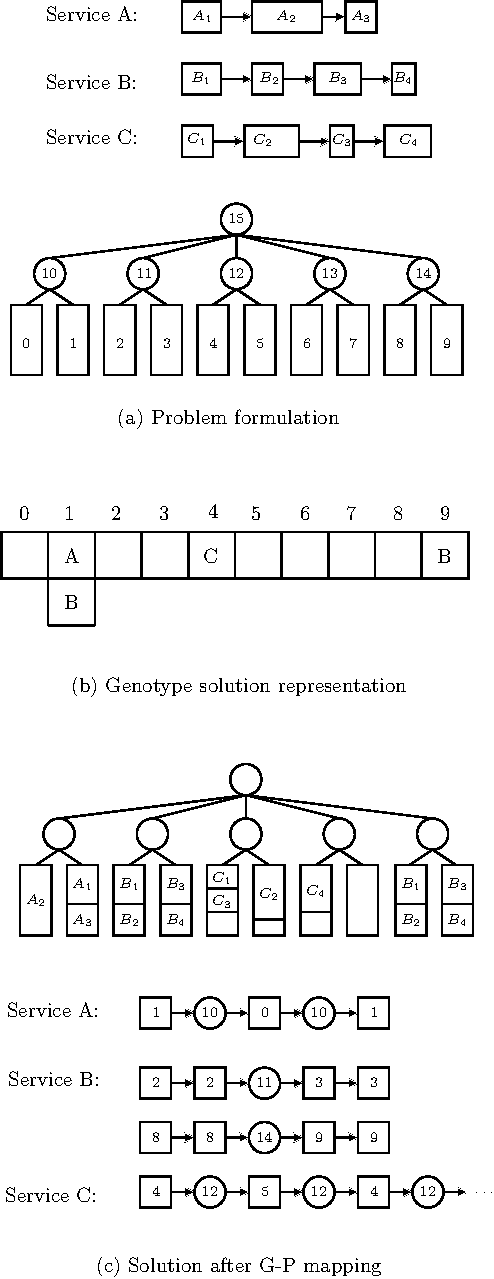
\includegraphics{figures/operators/mapping-crop}
    \caption{An example of the components of the solution representation.}
    \label{fig:mapping}
\end{figure}

% TODO: Heading sentences are still tricky here

One of the key challenges when designing an EA for real-world problems is selecting the right solution representation. For complex problems such as the VNFPP, it can be beneficial to introduce domain knowledge into the solution representation to improve the expected solution quality. One way this can be performed is using a \textit{genotype-phenotype} (G-P) solution representation. A G-P solution representation defines a `genotype' solution representation ($\Omega'$) and a G-P mapping function to convert it into the true solution space, f:$\Omega' \implies \Omega$. Domain knowledge can be introduced into the genotype and in the G-P mapping function.

In this work we use a G-P solution representation to improve the probability of generating a feasible solution and to minimize the distance between sequential VNFs. The genotype is a list of servers where each server can contain any number of \textit{service instances} - an indicator that a service should start from that location. \pref{fig:mapping} illustrates how the G-P mapping is performed. The mapping algorithm iterates over each service instance, and maps each VNF of the service to the nearest server that can accommodate it (\pref{fig:mapping} iii). Once all VNFs have been placed, the mapping then finds the set of shortest paths between the VNFs of the service and assigns them to the solution (\pref{fig:mapping} iv).

\begin{algorithm}[t!]
	
    % TODO: All these terms need standardising

	\KwData{Initial server $s$, cache size $n_{max}$}
	\KwResult{Server distance cache $C_s$}

    $C_s \gets \emptyset$
    
    $Q_c \gets {s}$ \tcp{Current horizon}

    $Q_n \gets \emptyset$ \tcp{Next horizon}

    $E \gets \emptyset$ \tcp{Explored nodes}

    \While{$Q_c \neq \emptyset$} {
        $u \gets \text{Get random element of } Q_c$

        $Q_c \gets Q_c \ u$
        
        \If{$u \text{ is a server}$}{
            $C_s \gets C_s \cup u$

            \If{$\abs{C_s} == n_{max}$} {
                \Return{$C_s$}
            }
        }

        \ForEach{$\text{neighbour } v $ \Of $u$}{
            \If{$v \notin E$}{
                $Q_n \gets Q_n \cup v$

                $E \gets E \cup v$
            }
        }

        \If{$Q_c = \emptyset$}{
            $Q_c \gets Q_n$

            $Q_n \gets \emptyset$
        }
    }

	\caption{A non-deterministic breadth first search algorithm.}
	\label{alg:nd_bfs}
\end{algorithm}

\begin{figure*}[t]
    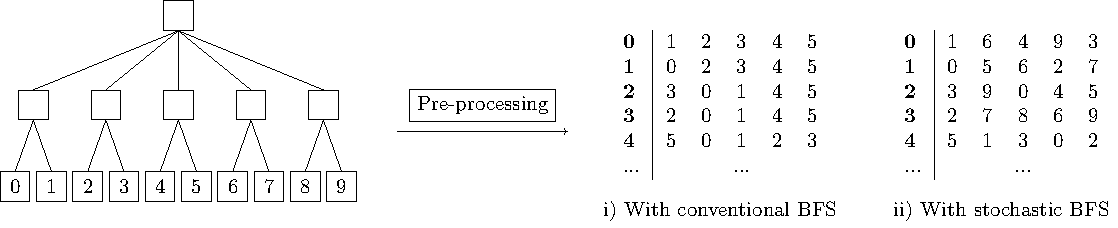
\includegraphics[width=\textwidth]{figures/operators/preprocessing}

    \caption{The results of generating the server cache with a conventional BFS vs a stochastic BFS}
    \label{fig:server_gen}
\end{figure*}

The G-P mapping function uses two preconstructed data structures to run efficiently: a set of routing tables for each network component and a set of distance tables for each server.
\begin{itemize}
    \item \textit{Distance tables} are used to find the next nearest server with sufficient capacity to place a VNF. Each distance tables simply list the other servers in the data center in increasing order of distance.
    \item \textit{Forwarding tables} are used to find the shortest routes between two servers. Each node in the graph has a forwarding table which can be consulted to find the next steps towards a server.
\end{itemize}

Naive implementations of these constructs do not scale well to large problems since the memory required scales with the number of servers and switches \cite{BillingsleyLMMG20}. In this work we propose compressed versions of both data structures for use on large problems.

\subsubsection{Distance table compression}
The distance tables can be constructed using breadth first search (BFS) which will encounter every other server in the data center in increasing order of distance. In a naive implementation, each distance table will store a reference to every other server, for a $O(n^2)$ total memory complexity across all distance tables. However, since the mapping procedure will only consult the table until it finds a suitable server, each table only needs to contain as many servers as are likely to be accessed.

The compressed version of the table can be crafted by simply halting the search early. However, if the distance tables do not contain all servers, a `cache miss' can occur if the mapping procedure does not find a suitable server in the distance table. As illustrated in \pref{fig:server_gen}, deterministic methods of identifying nearby servers such as BFS can accentuate this issue as a small number of servers will be overrepresented on average. 

We resolve this issue using a non-deterministic BFS (\pref{alg:nd_bfs}). The non-deterministic BFS modifies the well known BFS by exploring the neighbors of the current frontier in a random order. Since nodes that are encountered earlier are still explored earlier, the nearest nodes to a server are still discovered first. However, all servers which are the same distance away are equally likely to appear in the distance table.

% Finally, the minimum length of the distance table is dependent on a number of factors such as the network topology, number of services and properties, tolerance for failure etc. This prevents a simple closed form expression for the minimum length of each distance tables. Instead, we adapt a monte-carlo method to find a setting that guarantees high reliability. 

\subsubsection{Forwarding table compression}
We create the forwarding tables using a modified version of the initialization process of the equal-cost multi-path (ECMP) routing protocol. In the first step, a server broadcasts a message listing its ID and the distance the message has travelled so far. Upon receiving a message, if the component has received a message for that server with a lower distance it will discard it. Otherwise it will record the origin of the message as one of the next steps to the server, increment the distance and rebroadcast the message. Once all network components have received a message from all servers, the algorithm terminates.

Due to the large number of servers and switches in a data center, it is infeasible to store uncompressed forwarding tables in memory. As data centers must support high numbers of servers each port must facilitate access to many servers. Hence, we can often aggregate several rules which list the same hops together into a single rule to save memory. 

In this work, we aggregate rules that pertain to servers with sequential IDs. Each rule specifies the range of servers it encompasses and the next hop for which any server in that range should take. We apply these compression rules for each forwarding table after each server broadcast occurs. 

The memory saving from this approach depends on the network topology. In the worst case, this approach has the same worst case memory complexity as the naive implementation. In practice however, we find it results in significant memory savings (see Section \ref{sec:evaluation}). 

% \begin{figure}
%     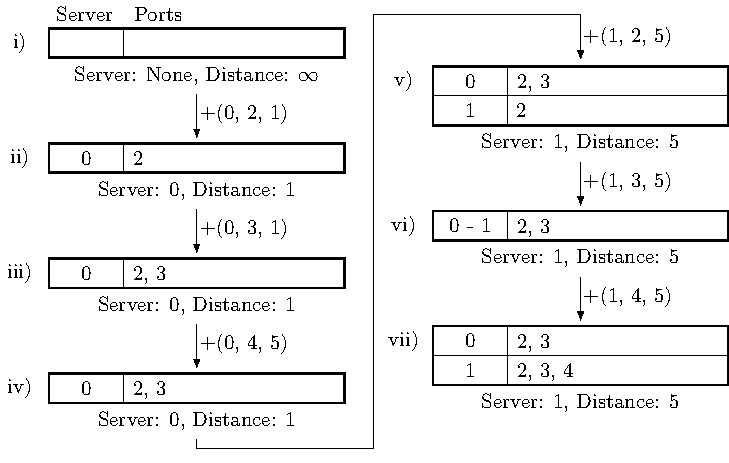
\includegraphics[width=\columnwidth]{figures/operators/routing_compression_three}
%     \caption{An example routing compression process. The tuple (server, edge, distance) denotes the server the message was originally sent from, the edge the message was received from and the distance to the server from that edge. The routing table keeps track of the edges that are on the shortest paths to each server.}
%     \label{fig:routing}
% \end{figure}

\subsection{Operators}
\label{sec:operators}
Finally we discuss the design of the operators used in this work. Our proposed metaheuristic requires two operators: an initialization operator that provides seed solutions to the subproblems and a neighbor generation operator that generates a solution in the neighborhood of a given solution and is an integral part of the local search procedure.

\subsubsection{Initialization}
\label{sec:initialization}
% - Context 
% - Motivation / Challenge
Good initial solutions can significantly improve the final quality of the solutions to single objective problems \cite{VlasicDJ19,RamseyG93,OsabaDCOL14} such as the subproblems in our algorithm. Since the weights are uniformly distributed over the objective space, it is important that the archive contains a diverse population. We designed an initialization operator that produces diverse initial solutions for the first archive in order to seed the search process with good initial solutions.

% In earlier work \cite{BillingsleyLMMG22}, we proposed a problem aware initialization technique that produced high quality and diverse solutions. However, the operator only produced solutions where there were the same number of instances of each service, causing parts of the objective space to be over represented. In this work we correct this restriction to produce better distributed solutions.

%%% - Solution
To ensure the population is diverse, we determine the minimum and maximum number of service instances the data center can accommodate and then generate solutions uniformly over this space. A feasible solution has at least one instance of each VNF, hence the minimum capacity that will be used is the sum of the size of all VNFs,

\begin{equation}
    M^\textsf{min} = \sum_{v\in \mathcal{V}} C_v
\end{equation}

\noindent Similarly, a solution cannot place more VNFs than there is capacity for, hence the maximum capacity is the total capacity of the data center,

\begin{equation}
    MD^\textsf{max} = n \cdot C^s
\end{equation}

\noindent Next, we determine how much capacity each solution should be allocated. For a population with $n$ individuals, we permit the $i$th individual to use at most $i / n$\% of the total capacity. The number of instances of each service is determined by:
\begin{equation}
    N_v^i = \left(M^\textsf{min}\ /\ M^\textsf{max} - 1 \right) \cdot \frac{i}{n} + 1.
\end{equation}
where the whole number part determines the guaranteed number of each instance whilst the fractional part determines the probability an additional instance is placed. This ensures that expected number of service instances meets the target capacity.

Once the number of instances of each service have been calculated, the service instances are distributed uniformly at random over the initial solution.

\subsubsection{Neighbor Generation}
\label{sec:local_search}
The local search procedure aims to find improving solutions by exploring the immediate neighborhood of a solution. The neighborhood of the VNFPP contains changes in the number and placement of service instances. To explore this space, our neighbor generation function has an equal probability to add or remove a service instance or to move a service instances to a new server.